%\documentclass[spanish]{beamer}
\documentclass{beamer}
\usepackage{pgf,pgfpages}
%\pgfpagesuselayout{4 on 1}[letterpaper,landscape,border shrink=0.5in]
\usepackage{algorithm,algorithmic}
%\usepackage{algorithm,algorithmicx}
%\usepackage[noend]{algpseudocode}
\usepackage{listings}
\lstset{basicstyle=\ttfamily,
	showstringspaces=false,
	commentstyle=\color{red},
	literate={á}{{\'a}}1
	{ã}{{\~a}}1
	{é}{{\'e}}1
	{É}{{\'E}}1
	{ó}{{\'o}}1
	{í}{{\'i}}1
	{ñ}{{\~n}}1
	{¡}{{!`}}1
	{¿}{{?`}}1
	{ú}{{\'u}}1
	{Í}{{\'I}}1
	{Ó}{{\'O}}1
}

\usepackage{beamerthemesplit}
\usepackage{color}
\usepackage[utf8]{inputenc}
\usepackage[spanish]{babel}
%\usepackage[latin1]{inputenc}
%\usepackage[pdftex]{graphicx}
%\usepackage{algorithm}
%\usepackage{algorithmic-C}
%\usepackage{algorithmic}
\usepackage{amsthm}
\usepackage{multicol}
\usepackage{multirow}
\usepackage{fancyvrb,relsize}
\usepackage{hhline}
\usepackage{tikz}
\usetikzlibrary{trees, shapes, calc}
\newcommand{\inputTikZ}[2]{%
	\scalebox{#1}{\input{#2}}
}

\usetheme{Warsaw} %Gueno
%\usetheme{Darmstadt} %OK!
% \usetheme{Frankfurt} %OK!
%\usetheme{Goettingen}
%\usetheme{Dresden}
%\usetheme{JuanLesPins} %OK!!
%\usetheme{Marburg}
%\usetheme{Montpellier}
%\usetheme{Rochester} %sobrio
%\usetheme{Singapore}
%\usetheme{Szeged}

%\usecolortheme{albatross}
%\usecolortheme{seahorse}
%\usecolortheme{beetle}
%\usecolortheme{crane}
%\usecolortheme{dolphin}
%\usecolortheme{dove}
%\usecolortheme{fly}
%\usecolortheme{lily} %Gueno
\usecolortheme{orchid}%Gueno
%\usecolortheme{rose}
%\usecolortheme{seagull}
%\usecolortheme{whale}


\DefineVerbatimEnvironment%
      {VerbatimNN}%
      {Verbatim}%
      {fontsize=\relsize{-1}}
\DefineVerbatimEnvironment%
      {VerbatimNNN}%
      {Verbatim}%
      {fontsize=\relsize{-2}}

\DefineVerbatimEnvironment%
      {VerbatimPseudo}%
      {Verbatim}%
      {numbers=left, fontsize=\relsize{-1}}
\DefineVerbatimEnvironment%
      {VerbatimPseudoReduced}%
      {Verbatim}%
      {numbers=left, fontsize=\relsize{-2}}
\DefineVerbatimEnvironment%
      {VerbatimPseudoReduced2}%
      {Verbatim}%
      {numbers=left, fontsize=\relsize{-3}}
\DefineVerbatimEnvironment%
      {VerbatimC}%
      {Verbatim}%
      {commandchars=@ªº, numbers=left, fontsize=\relsize{-1}}
\DefineVerbatimEnvironment%
      {VerbatimReducedC}%
      {Verbatim}%
      {commandchars=@ªº, numbers=left, fontsize=\relsize{-2}}
\DefineVerbatimEnvironment%
      {VerbatimReduced2C}%
      {Verbatim}%
      {commandchars=@ªº, numbers=left, fontsize=\relsize{-3}}



%\AtBeginSubsection[]
%{
% \begin{frame}
% \frametitle{Sinopsis}
% Aqui decides: cada seccion y subseccion:
% \tableofcontents[currentsection,currentsubsection]
 %O solamente la seccion (Solo uno de ellos)
%\tableofcontents[currentsection]
% \end{frame}
%}

% Si quieres que todo por default aparezca de poco en poco
% descomenta esta linea
%\beamerdefaultoverlayspecification{<+->}

\setbeamertemplate{footline}{\hfill\insertframenumber/\inserttotalframenumber}
\setbeamertemplate{navigation symbols}{}

\setbeamercovered{transparent}

\title{ELO320 - Estructuras de Datos y Algoritmos\\Análisis de Complejidad\\\small{Insertion Sort}}
%\subtitle{Ingeniería Civil Telemática UTFSM}
\author{Dr. Nicolás Gálvez R.\\{\small nicolas.galvez@usm.cl}}
\institute{Ing. Civil Telemática - Departamento de Electrónica}
\titlegraphic{
\includegraphics[scale=.18]{images/logoutfsm}}
\date{2do Semestre 2022}

\begin{document}

\frame{\titlepage}

%\section*{Sinopsis}
%\frame{  \frametitle{Sinopsis}\tableofcontents[pausesections]}
%
%

\section{Análisis de Complejidad}
\begin{frame}[fragile]
 \frametitle{Complejidad en Algoritmos}
\small
\textbf{¿Cómo podemos comparar dos algoritmos que resuelven un mismo problema?}

\begin{itemize}
\item Opción 1: programar ambos y ver cuántos recursos computacionales consumen. Pero:
\begin{itemize}
\item Poco eficiente en costo $\rightarrow$ sólo uno será utilizado. 
\item Algún algoritmo puede ser mal implementado $\rightarrow$ se subestima.
\item Casos de prueba pueden favorecer a algún algoritmo en específico.
\item Ambos algoritmos pueden ser muy costosos de implementar.
\end{itemize}
\smallskip
\item Opción 2: Análisis de Algoritmo $\rightarrow$ Análisis de Tiempo de Ejecución.
\item Opción 3: Análisis Asintótico.
\end{itemize}
\end{frame}


\begin{frame}[fragile]
 \frametitle{Complejidad en Algoritmos}
\small
\begin{itemize}
\item Medir eficiencia $\rightarrow$ entrada de tamaño creciente ($n \rightarrow \infty$). 
\item Técnicas de estimación del costo.
\item Definir costos de un algoritmo antes de implementarlo.
\end{itemize}

\begin{block}{Algoritmo}
\medskip
\centering Entrada $\rightarrow$ Procedimiento $\rightarrow$ Salida.
\medskip
\end{block}

Se miden por recursos utilizados:
\begin{itemize}
\item Tiempo.
\item Memoria.
\item Ancho de Banda usado.
\end{itemize}
\end{frame}


\begin{frame}[fragile]
 \frametitle{Complejidad en Algoritmos}
\small
\begin{itemize}
\item Medir eficiencia $\rightarrow$ entrada de tamaño creciente ($n \rightarrow \infty$).
\item Técnicas de estimación del costo.
\item Definir costos de un algoritmo antes de implementarlo.
\end{itemize}

\begin{block}{Algoritmo}
\medskip
\centering Entrada $\rightarrow$ Procedimiento $\rightarrow$ Salida.
\medskip
\end{block}

Se miden por recursos utilizados:
\begin{itemize}
\item \textbf{Tiempo.}
\item Memoria.
\item Ancho de Banda usado.
\end{itemize}
\end{frame}

\begin{frame}[fragile]
 \frametitle{Complejidad en Algoritmos}
\small El tiempo de un algoritmo varía según donde sea implementado. Por esta razón, nos referiremos a los siguientes elementos (normalizados):

\begin{itemize}
\item Cantidad de accesos a la memoria.
\item Número de comparaciones
\item Cantidad de veces que se ejecuta un ciclo.
\end{itemize}
Esto se resume en:
\begin{block}{Complejidad en tiempo}
\medskip
\centering \textbf{Nº de operaciones realizadas} $\times$ \textbf{Costo de cada operación}.
\medskip
\end{block}
\end{frame}

\begin{frame}[fragile]
 \frametitle{Complejidad en Algoritmos}
\begin{block}{Complejidad en tiempo}
\medskip
\centering \textbf{Nº de operaciones realizadas} $\times$ \textbf{Costo de cada operación}.
\medskip
\end{block}

Utilizaremos una medida estándar (\textit{ceteris paribus}):
\begin{center} \textbf{Costo de cada operación} $\rightarrow$ \textbf{1}. \end{center}
\medskip

Esto debido a que una plataforma con mejor características producirá que un mismo algoritmo tenga mejor desempeño respecto a otra plataforma.
\end{frame}



\begin{frame}[fragile]
 \frametitle{Tiempo de ejecución de un Algoritmo}
\small Definiremos $T(n)$ como la función de tiempo de ejecución de un algoritmo con input $n$, y la expresaremos en función a la cantidad de instrucciones.\\
\bigskip
Costo de las operaciones en unidades de tiempo [ut]:
\begin{itemize}
\item Instrucciones básicas: $1$
\item Secuencia de $n$ instrucciones:  $c \times n = n$ (c: cte. de costo)
\item if-else: $T(\text{condición}) + \text{max}\{T(\text{if}), T(\text{else})\}$
\item while: $(n+1) \times T(\text{condición}) + n \times T(\text{while}) $
\end{itemize}
\end{frame}


\begin{frame}[fragile]
 \frametitle{Tiempo de ejecución de un Algoritmo}
\begin{exampleblock}{¿Cuál es la complejidad del siguiente algoritmo?}
\begin{lstlisting}[language=C, basicstyle=\tiny, escapeinside={|}{|}, numbers=left]
int suma(int n) {
	int sum = 0, i, j;
	for (i=0; i < n; i++) 
		for (j=0; j < n; j++)
			sum++;
	return sum;
}
\end{lstlisting}
\end{exampleblock}
\pause
\begin{itemize}
\item Orden del número de iteraciones: $n^2$. \pause
\begin{itemize}
\item Costo L.2: \pause 3. \pause 
\item Costo cada for (L.3, L.4): \pause $1+(n+1)+n = 2n+2$. \pause
\item Costo L.5: \pause 1. \pause
\item Costo L.6: \pause 1. \pause
\end{itemize}
\item Costo for interno (L.4 + L.5):  \pause $2n+2+n = 3n+2$. \pause
\item Costo de doble for (L.3 + L.4 + L.5): \pause $(2n+2) \times (3n+2) = 6n^2 + 10n + 4$. \pause
\item Costo total: \pause $6n^2 + 10n + 8$. \pause
\end{itemize}

\end{frame}


\begin{frame}[fragile]
 \frametitle{Complejidad Algorítmica vs Entorno de ejecución.}
\small
Los primeros algoritmos de ordenamiento que veremos son:
\begin{itemize}
\item \textbf{Insert Sort}: $T_1(n) = c_1 \times n^2$
\item \textbf{Merge Sort}: $T_2(n) = c_2 \times n \times \log{n}$
\end{itemize}

Supongamos que el PC-A está ejecutando \textbf{Insert Sort}, que el PC-B está ejecutando \textbf{Merge Sort} y que ambos deben ordenar un arreglo de 10 millones de enteros.
Además, el PC-A es de última generación y ejecuta 10 mil millones de instrucciones por segundo y el PC-B tiene 10 años de antigüedad y sólo procesa 10 millones de instrucciones por segundo.
Incluyamos lo siguiente:
\begin{itemize}
\item Julio Profe programó \textbf{Insert Sort} en el PC-A usando lenguaje de máquina (assembly) resultando en un costo de $2\times n^2$ instrucciones para ordenar n números.
\item El Corxea implementa \textbf{Merge Sort}, en el PC-B usando C++, con un compilador antiguo e ineficiente, y el código resultante toma $50 \times n \times \log{n}$ instrucciones para ordenar n números.
\end{itemize}

\end{frame}


\begin{frame}[fragile]
 \frametitle{Complejidad Algorítmica vs Entorno de ejecución.}
\small

\begin{itemize}
\item PC-A:
$$ \frac{2 \times (10^7)^2}{10^{10}} = 20000\ [s]\ \ (>5.5 [h])$$
\item PC-B:
$$ \frac{50 \times 10^7 \times \log{10^7}}{10^{7}} \approx 1163\ [s]\ \ (< 20 [min])$$
\end{itemize}
\bigskip
\textbf{PC-B completa su algoritmo 17 veces más rápido que el algoritmo usado en PC-A, siendo el segundo entorno de ejecución 1000 veces más lento que el primero}.

\end{frame}

\begin{frame}[fragile]
 \frametitle{Complejidad Algorítmica vs Entorno de ejecución.}
\small

\begin{center}
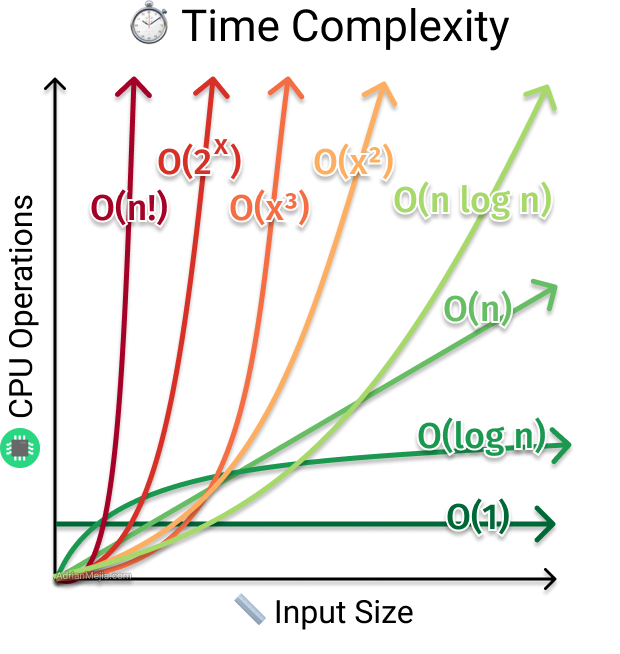
\includegraphics[width=.7\linewidth]{images/timecomplexity2}
\end{center}


\end{frame}


\section{Análisis Asintótico}

\begin{frame}[fragile]
 \frametitle{Análisis Asintótico}
\small Una vez entendido el análisis de tiempo buscaremos análisis asintótico de los algoritmos. En la práctica significa concentrarse en el término predominante en $T(n)$, y luego encontrar cotas de rendimiento.
\medskip

Existen tres notaciones asintóticas generalmente usadas:
\begin{itemize}
\item Big O ($\mathcal{O}$): Cota superior asintótica, vale decir, cota al peor desempeño.
\item Big Omega ($\Omega$): Cota inferior asintótica, vale decir, cota al mejor desempeño.
\item Big Theta ($\Theta$): Cota compuesta, vale decir, cota al rendimiento promedio. 
\end{itemize}
\medskip

Comúnmente, se utiliza la notación en peor escenario, vale decir, Big O ($\mathcal{O}$). 
\end{frame}

\begin{frame}[fragile]
 \frametitle{Análisis Asintótico: Big O ($\mathcal{O}$)}
\small Cota asintótica que limita el peor desempeño de un algoritmo.

\begin{exampleblock}{Big O ($\mathcal{O}$)}\small
Sean $f$ y $g$ dos funciones en $\mathbb{R}$, diremos que:
$$f(n) = \mathcal{O}(g(n)) \iff f(n) \in \mathcal{O}(g(n))$$
Donde:
$$ \mathcal{O}(g(n)) = \{f(n)\ |\ \exists c \in \mathbb{R}, f(n) \leq c \times g(n);\ \forall n \geq n_0\}$$
\end{exampleblock}

\begin{center}
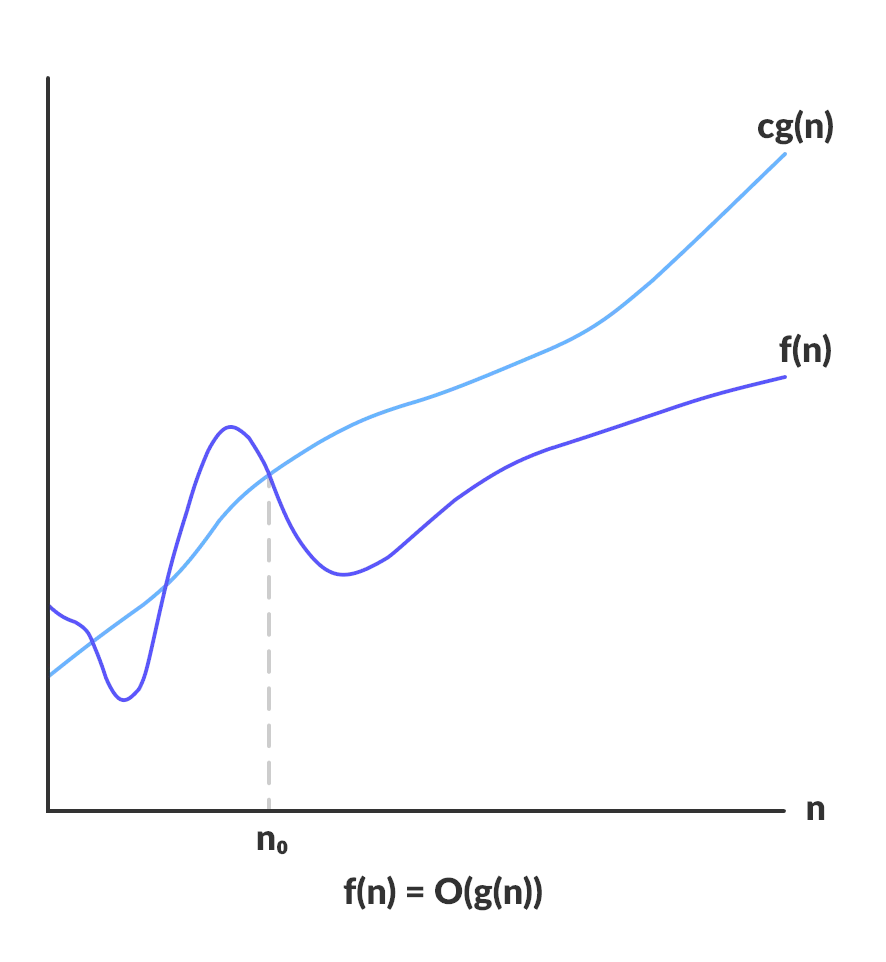
\includegraphics[width=.35\linewidth]{images/bigO}
\end{center}

\end{frame}

\begin{frame}[fragile]
 \frametitle{Análisis Asintótico: Big Omega ($\Omega$)}
\small Cota asintótica que limita el mejor desempeño de un algoritmo.

\begin{exampleblock}{Big Omega ($\Omega$)}\small
Sean $f$ y $g$ dos funciones en $\mathbb{R}$, diremos que:
$$f(n) = \Omega(g(n)) \iff f(n) \in \Omega(g(n))$$
Donde:
$$ \Omega(g(n)) = \{f(n)\ |\ \exists c \in \mathbb{R},  c \times g(n) \leq f(n) ;\ \forall n \geq n_0\}$$
\end{exampleblock}

\begin{center}
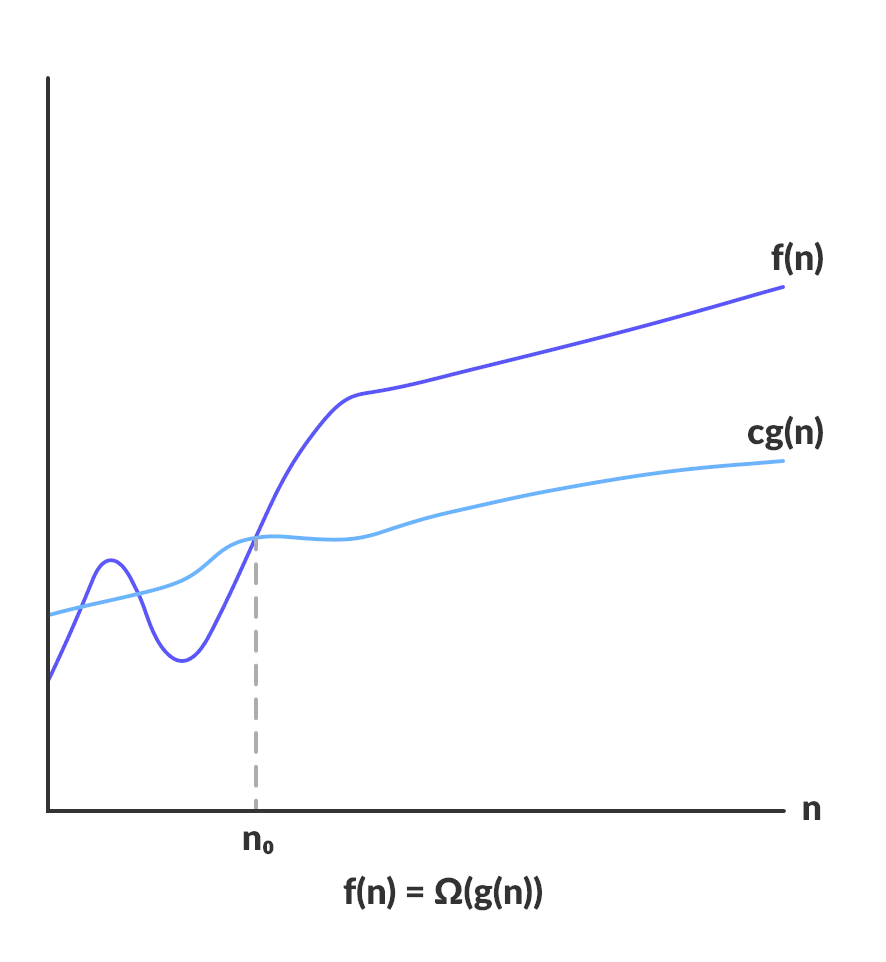
\includegraphics[width=.35\linewidth]{images/bigOmega}
\end{center}

\end{frame}

\begin{frame}[fragile]
 \frametitle{Análisis Asintótico: Big Theta ($\Theta$)}
\small Cota asintótica que limita el desempeño promedio de un algoritmo.

\begin{exampleblock}{Big Theta ($\Theta$)}\small
Sean $f$ y $g$ dos funciones en $\mathbb{R}$, diremos que:
$$f(n) = \Theta(g(n)) \iff f(n) \in \Theta(g(n))$$
Donde:
$$ \Theta(g(n)) = \{f(n)\ |\ \exists (c_1, c_2) \in \mathbb{R}^2, c_1 \times g(n) \leq f(n) \leq c_2 \times g(n);\ \forall n \geq n_0\}$$
\end{exampleblock}

\begin{center}
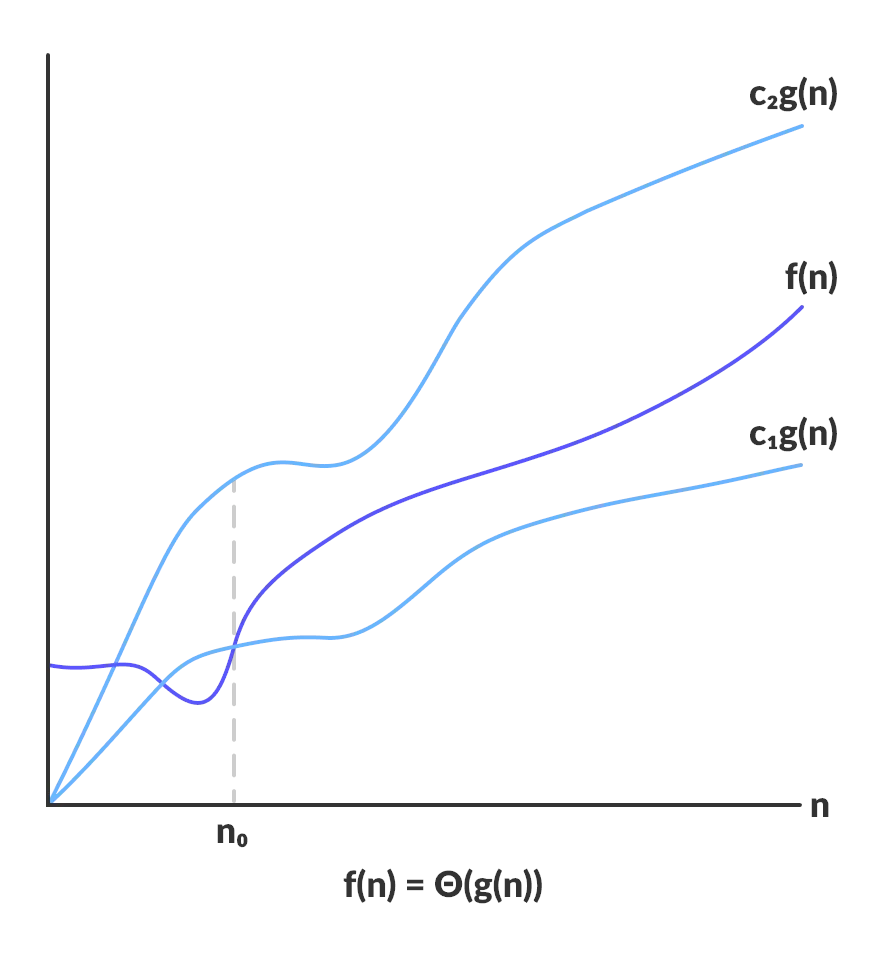
\includegraphics[width=.35\linewidth]{images/bigTheta}
\end{center}

\end{frame}

\begin{frame}[fragile]
 \frametitle{Análisis Asintótico}
\begin{exampleblock}{¿Cuál es la complejidad del siguiente algoritmo}
\begin{lstlisting}[language=C, basicstyle=\tiny, escapeinside={|}{|}]
int suma(int n) {
	int sum = 0, i, j;
	for (i=0; i < n; i++) 
		for (j=0; j < n; j++)
			sum++;
	return sum;
}
\end{lstlisting}
\end{exampleblock}
\small
\pause
\begin{itemize}
\item Costo total $f(n) =$ \pause $6n^2 + 10n + 8 $.
\item $g(n) = n^2$, termino del grado superior.
\item Cota superior: \texttt{suma} $= \mathcal{O}(n^2)$ \pause $\rightarrow$ \pause $f(n) \leq 10 \times g(n) $
\item Cota inferior: \texttt{suma} $= \Omega(n^2)$ \pause $\rightarrow$ \pause $3 \times g(n) \leq f(n) $
\item Cota promedio: \texttt{suma} $= \Theta(n^2)$ \pause $\rightarrow$ \pause $3 \times g(n) \leq f(n) \leq 10 \times g(n)$
\end{itemize}
\end{frame}

\begin{frame}[fragile]
 \frametitle{Análisis Asintótico}
\small
\begin{center}
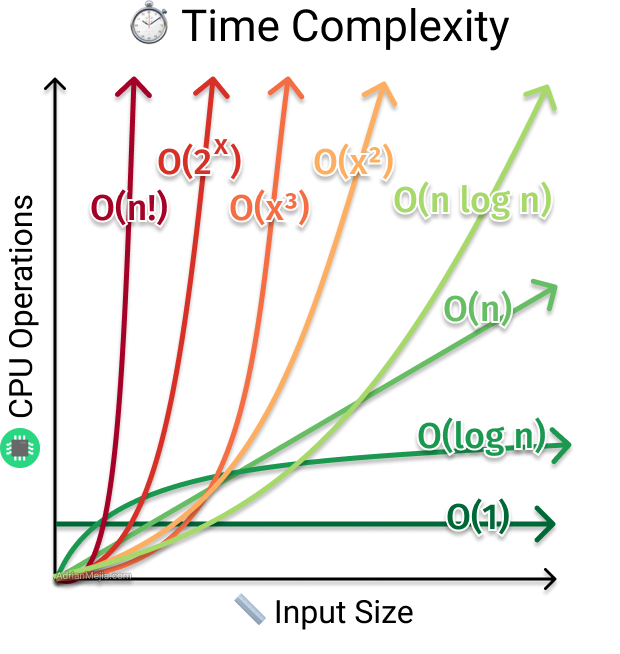
\includegraphics[width=.7\linewidth]{images/timecomplexity2}
\end{center}
\end{frame}


\begin{frame}[fragile]
 \frametitle{Análisis Asintótico}
\small
\begin{center}
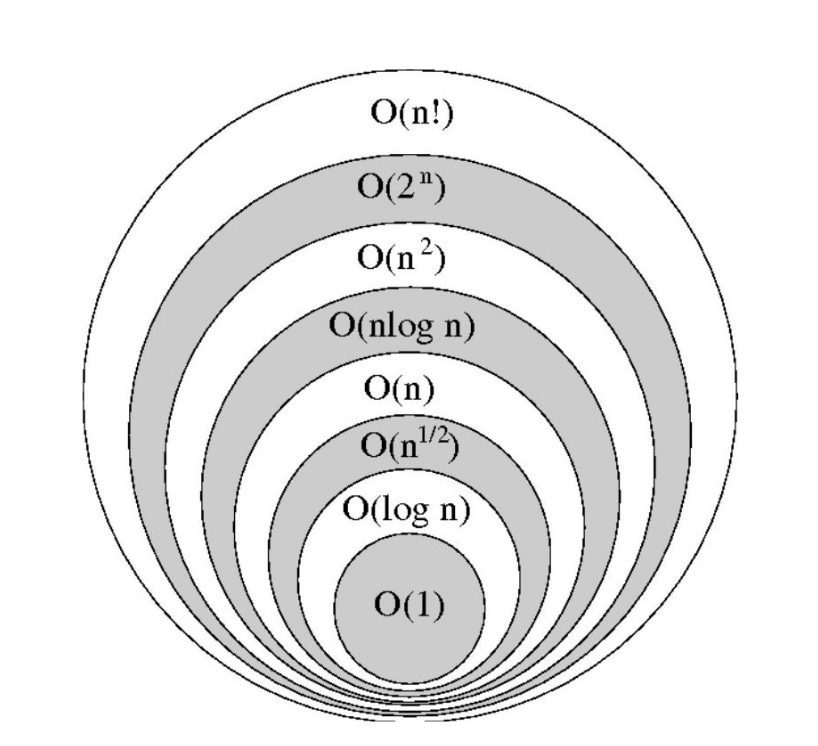
\includegraphics[width=.7\linewidth]{images/bigO2}
\end{center}
\end{frame}

\section{Insertion Sort}
\begin{frame}[fragile]
 \frametitle{InsertSort}
\small Es un método de ordenamiento de elementos, en el cual a través de la visitas de subconjuntos, un elemento es \textbf{insertado} en la posición ordenada que le corresponde.

\begin{center}
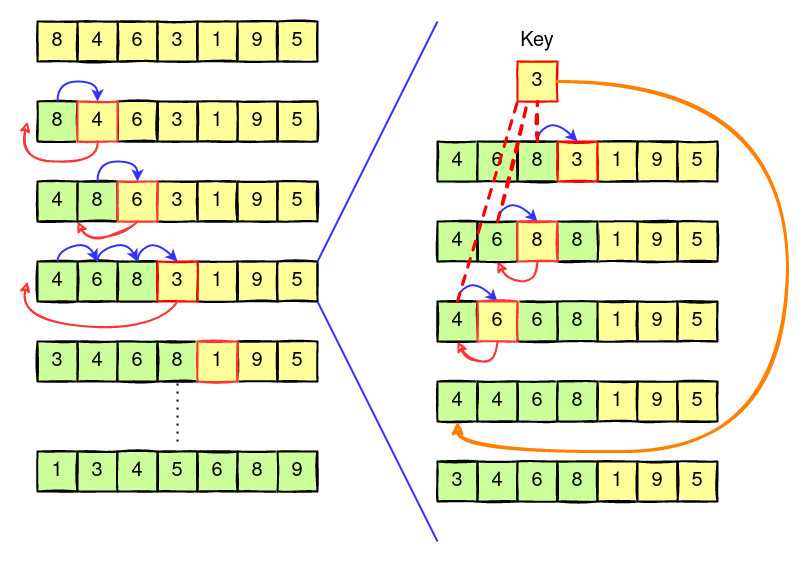
\includegraphics[width=.7\linewidth]{images/InsertSort}
\end{center}
\end{frame}

\begin{frame}[fragile]
 \frametitle{InsertSort}
\begin{exampleblock}{¿Cuál es la complejidad del siguiente algoritmo}
\begin{lstlisting}[language=C, basicstyle=\tiny, escapeinside={|}{|}]
void insertionSort(int arr[], int n){
	int i, key, j;
	for (i = 1; i < n; i++) {
		key = arr[i];
		j = i - 1;
 		while (j >= 0 && arr[j] > key) { //esto puede ser un for
			arr[j + 1] = arr[j];
			j--;
		}
        	arr[j + 1] = key;
    	}
}
\end{lstlisting}
\end{exampleblock}
\end{frame}

\begin{frame}[fragile]
 \frametitle{InsertSort: Complejidad}

\begin{itemize}
\item Cota Superior: $\mathcal{O}(n^2) \rightarrow$ Caso peor: todo invertido. 
\item Cota Inferior: $\Omega(n) \rightarrow$ Mejor caso: todo ordenado.
\item Cota Promedio: $\Theta(n^2) \rightarrow$ Caso promedio para arreglos aleatorios. 
\end{itemize}

Extrapolando a otros algoritmos, ¿Por qué generalmente se usa $\mathcal{O}$ y no $\Theta$? Debido a que en muchos algoritmos, $\Theta$ no es sostenible para TODOS los casos.

\end{frame}

\begin{frame}[fragile]
 \frametitle{Ejercicios}
\small
\begin{itemize}
\item Revisite las implementaciones de listas, pilas, colas y árboles y determine la complejidad de sus métodos.
\item Mostrar la evolución de Insert Sort en el arreglo A = {31, 41, 59, 26, 41, 58}
\item Reescribir Insert Sort para ordenamiento de datos de manera decreciente.
\item Expresar la ecuación $n^3/1000 - 100n^2 - 100n + 3$ en términos de notación asintótica.
\item Considere el problema de sumar dos números enteros expresados base binaria, almacenados en dos arreglos A y B de n elementos (bits) cada uno. La suma de los dos enteros se debe almacenar en forma binaria en un arreglo C de (n+1) elementos. Escriba una función en C para la suma los dos enteros. ¿Qué complejidad tiene su función? Compárela con la de sus compañeros.
\end{itemize}


\end{frame}

%\begin{frame}[fragile]
% \frametitle{ABB: Árbol binario de búsqueda}
%\small
%Por ejemplo, es fácil determinar el lugar y posición de los valores en un intervalo. 
%
%\begin{center}
%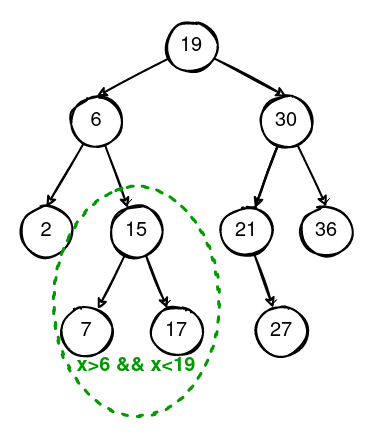
\includegraphics[width=.35\linewidth]{images/abb3}
%\end{center}
%
%\begin{itemize}
%\item \textbf{¿Cómo determinan el sucesor y predecesor de un padre?}\\
%{\color{red}{Sucesor: buscar en la derecha, todo hacia la izquierda.}}\\
%{\color{blue}{Antecesor: buscar en la izquierda, todo hacia la derecha.}} \\
%\item \textbf{¿Cuál es su principal característica?}\\
%{\color{red}{Siempre tendrán a lo más un hijo.}}
%\end{itemize}
%\end{frame}
%
%
%\begin{frame}[fragile]
% \frametitle{ABB: Operaciones}
%\small Las operaciones más comunes de los ABB son:
%
%\begin{itemize}
%\item \texttt{init()}: Inicializar el árbol (root == NULL).
%\item \texttt{size()}: Cantidad de elementos en el árbol.
%\item \texttt{x\_preorden()}: Operación x en pre-orden.
%\item \texttt{x\_inorden()}: Operación x en in-orden. 
%\item \texttt{x\_postorden()}: Operación x en post-orden. 
%\item \texttt{search()}: Buscar un elemento en el árbol.
%\item \texttt{insert()}: Insertar un elemento en el árbol.
%\item \texttt{delete()}: Eliminar un elemento en el árbol.
%\item \texttt{clear()}: Limpiar el árbol.
%\end{itemize}
%\end{frame}
%
%\begin{frame}[fragile]
% \frametitle{ABB: Recorrer}
%\small
%¿Como se imprimirían los datos del siguiente árbol con recorrido pre-orden, in-orden y post-orden?
%
%\begin{center}
%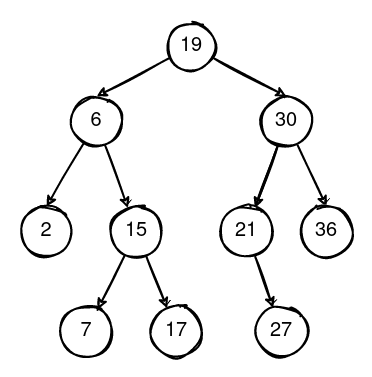
\includegraphics[width=.45\linewidth]{images/abb1}
%\end{center}
%
%\pause
%\begin{itemize}
%\item Pre-orden: 19 - 6 - 2 - 15 - 7 - 17 - 30 - 21 - 27 - 36 \pause
%\item In-orden: 2 - 6 - 7 - 15 - 17 - 19 - 21 - 27 - 30 - 36 \pause
%\item Post-orden: 2 - 7 - 17 - 15 - 6 - 27 - 21 - 36 - 30 - 19 
%\end{itemize}
%
%
%\end{frame}
%
%
%\begin{frame}[fragile]
% \frametitle{ABB: Buscar}
%Comenzaremos con la función básica \texttt{search()}: Buscar un elemento en el árbol.
%
%\begin{center}
%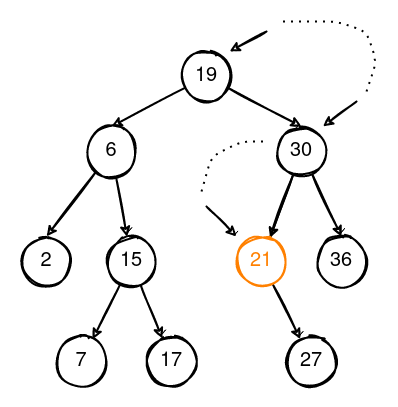
\includegraphics[width=.35\linewidth]{images/abb-search}
%\end{center}
%
%Se puede hacer de dos formas:
%\begin{itemize}
%\item Usando un puntero para recorrer el árbol.
%\item \textbf{Recursivamente}.
%\end{itemize}
%\end{frame}
%
%\begin{frame}[fragile]
% \frametitle{ABB: Buscar}
%
%\begin{exampleblock}{Recursivamente}
%\begin{lstlisting}[language=C, basicstyle=\tiny, escapeinside={|}{|}]
%int * search(nodo_t * raiz, int value){ 
%
%	if(raiz == NULL || raiz->dato == value) //{} omitidas
%		return raiz;
%	else if(value < raiz->dato)
%		return search(raiz->hijo_izq, value);
%	else if(value > raiz->dato) // else
%		return search(raiz->hijo_der, value);
%	
%}
%\end{lstlisting}
%\end{exampleblock}
%
%\begin{block}{Usando Puntero}
%\begin{lstlisting}[language=C, basicstyle=\tiny, escapeinside={|}{|}]
%int * search(nodo_t * raiz, int value){
%	
%	nodo_t * rec = raiz;
%	while(rec!=NULL){
%		if(rec->dato == value){
%			return rec;
%		}else if(value < rec->dato){
%			rec = rec->hijo_izq;
%		}else if(value > rec->dato){
%			rec = rec->hijo_der;
%		}
%	return rec; // NULL si no lo encuentra o arbol vacío
%}
%\end{lstlisting}
%\end{block}%
%\end{frame}
%
%\begin{frame}[fragile]
% \frametitle{ABB: Insertar}
%\small
%Para poder insertar debemos buscar primero el lugar donde debe realizarse la inserción. La idea es \textbf{mantener} el orden de nuestro ABB.
%
%\begin{center}
%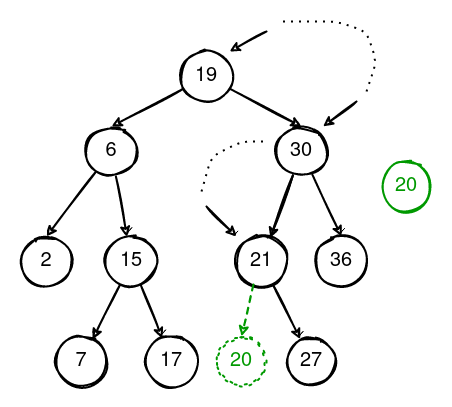
\includegraphics[width=.45\linewidth]{images/abb-insert}
%\end{center}
%
%Nota: Si nuestro árbol no acepta elementos repetidos, al encontrar el valor se detiene.
%
%\end{frame}
%
%\begin{frame}[fragile]
% \frametitle{ABB: Insertar}
%\begin{exampleblock}{Recursivamente}
%\begin{lstlisting}[language=C, basicstyle=\tiny, escapeinside={|}{|}]
%void insert(nodo_t ** raiz, int value){ 
%
%	if(*raiz == NULL){
%		*raiz = malloc(sizeof(node_t));
%		(*raiz)-> dato = value;
%		(*raiz)->hijo_izq = NULL;
%		(*raiz)->hijo_der = NULL;
%
%	}else if(value < (*raiz)->dato){
%		insert(&((*raiz)->hijo_izq), value);
%
%	}else if(value > (*raiz)->dato){
%		insert(&((*raiz)->hijo_der), value);
%	}
%}
%\end{lstlisting}
%\end{exampleblock}
%\end{frame}
%
%\begin{frame}[fragile]
% \frametitle{ABB: Insertar}
%Cree el árbol binario que represente la siguiente secuencia de enteros: 
%$$ 10 - 5 - 7 - 14 - 12 - 18 - 15 $$\pause
%\begin{alertblock}{Spoiler}
%\begin{center}
%\visible<.(1)>{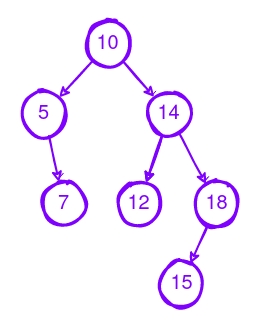
\includegraphics[width=.35\linewidth]{images/abb-insert-example}}
%\end{center}
%\end{alertblock}
%\end{frame}
%
%\begin{frame}[fragile]
% \frametitle{ABB: Eliminar}
%\small
%Al igual que en insertar, deberemos buscar el nodo a eliminar. Pero para poder eliminarlo, tendremos que considerar los siguientes casos:
%
%\begin{itemize}
%\item Nodo objetivo es una hoja (no tiene hijos).
%\item Nodo objetivo tiene un sólo hijo.
%\item Nodo objetivo tiene dos hijos.
%\end{itemize}
%
%\end{frame}
%
%\begin{frame}[fragile]
% \frametitle{ABB: Eliminar hoja.}
%\small
%Es el caso más sencillo, solo corresponde a liberar el nodo desde el puntero del padre.
%
%\begin{center}
%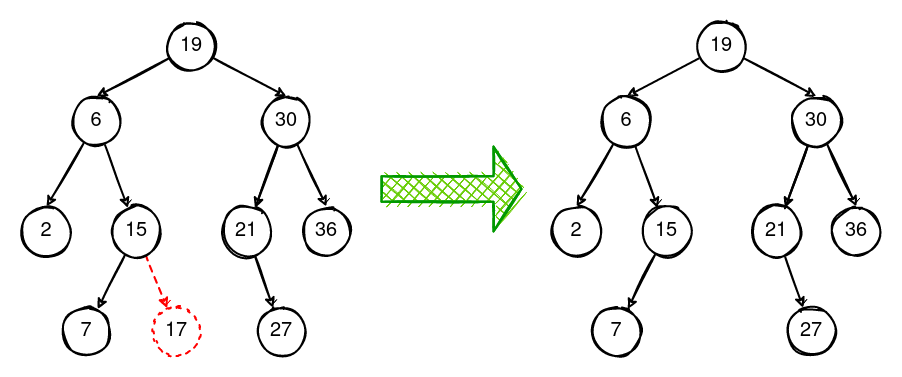
\includegraphics[width=.9\linewidth]{images/abb-delete-nochild}
%\end{center}
%\end{frame}
%
%\begin{frame}[fragile]
% \frametitle{ABB: Eliminar nodo con 1 hijo.}
%\small
%Caso intermedio. acá se elimina el nodo encontrado, pero su posición es ocupada por su único hijo. Se eleva ese sub-árbol, un nivel.
%
%\begin{center}
%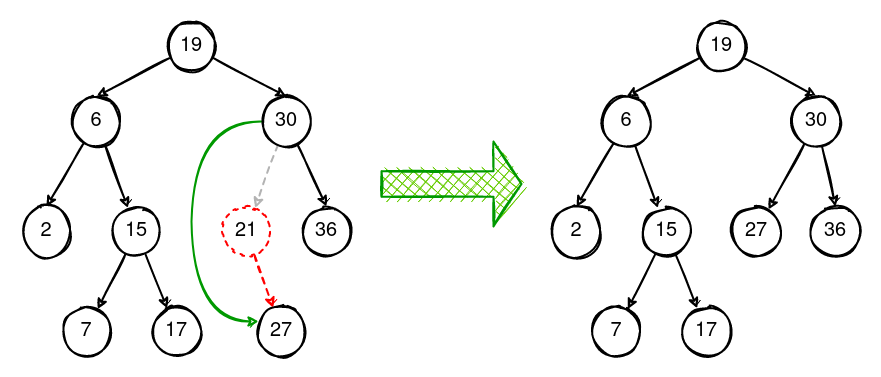
\includegraphics[width=.9\linewidth]{images/abb-delete-onechild}
%\end{center}
%\end{frame}
%
%\begin{frame}[fragile]
% \frametitle{ABB: Eliminar nodo con 2 hijos.}
%\small
%Caso recursivo o iterativo. Cuenta de dos pasos:
%\begin{itemize}
%\item Reemplazar el nodo objetivo por una copia de su sucesor o antecesor (uds. eligen).
%\item Borrar el sucesor o antecesor original.
%\end{itemize}
%
%\begin{center}
%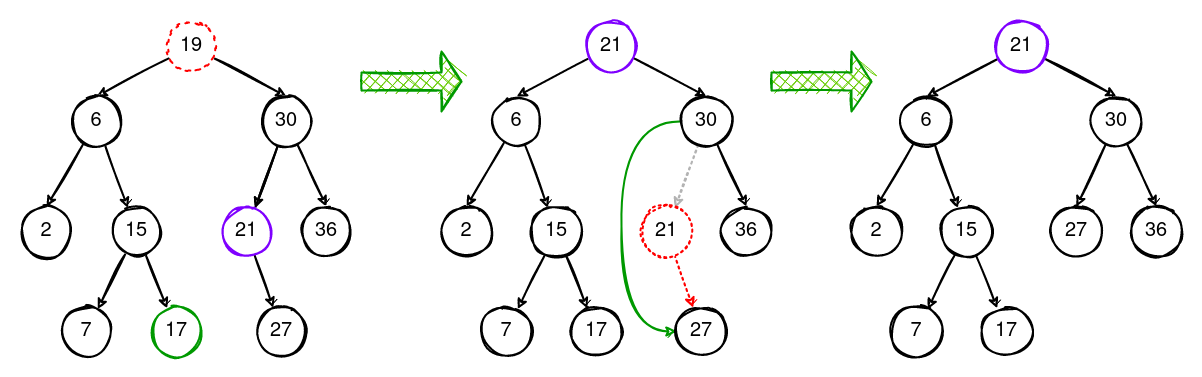
\includegraphics[width=\linewidth]{images/abb-delete-twochild}
%\end{center}
%\end{frame}
%
%
%
%\begin{frame}[fragile]
% \frametitle{ABB: Insertar}
%\begin{exampleblock}{Recursivamente}
%\begin{lstlisting}[language=C, basicstyle=\tiny, escapeinside={|}{|}]
%int delete(nodo_t ** raiz, int value){ 
%	// ¿Cómo lo programan?
%	// Necesitarán alguna función extra.
%}
%\end{lstlisting}
%\end{exampleblock}
%\end{frame}
%
%\begin{frame}[fragile]
% \frametitle{Ejercicios}
%\begin{itemize}
%\item Para el siguiente conjunto $\{1, 4, 5, 10, 16, 17, 21\}$, dibuje árboles binarios de búsqueda con altura 2, 3, 4, 5, y 6.
%\item Escriba funciones recursivas para recorrer un árbol binario de búsqueda en pre-orden y post-orden.
%\item Asuma que tiene números entre 1 y 1000 en un árbol binario de búsqueda y quiere buscar el nodo 363. ¿Cuál de las siguientes secuencias de nodos NO podría ser una secuencia de nodos examinados en el árbol para llegar al nodo 363?
%\begin{enumerate}
%\item 2, 252, 401, 398, 330, 344, 397, 363.
%\item 924, 220, 911, 244, 898, 258, 362, 363.
%\item 925, 202, 911, 240, 912, 245, 363.
%\item 2, 399, 387, 219, 266, 382, 381, 278, 363.
%\item 935, 278, 347, 621, 299, 392, 358, 363.
%\end{enumerate}
%\end{itemize}
%\end{frame}

\end{document}
